\section{Monopolios}

Es una firma que no enfrenta competencia. Esto genera mercados monopólicos que se producen naturalmente en servicios básicos, en firmas tecnológicas o en productos altamente innovadores. (e.g. proveedor de internet en un pueblo)\\

Estos no son socialmente eficientes.
\subsection{Curva de demanda}
Indica como varía la cantidad demandada de un bien cuando varía su precio. Tiene pendiente negativa.\\

Se escribe como una función $Q_D = Q_D(P)$. Sin embargo, al graficarlas se considera $Q$ como el eje horizontal y $P$ como el eje vertical.\\

\subsection{Función de utilidad}
Es la del proveedor o firma, se denota como $\Pi(Q)$, donde $Q$ representa la cantidad de demandada.

En general una firma monopólica observa una curva de demanda que le permite elegir entre distintas combinaciones de precio y cantidad, y obtener ingresos según ello.

\[\text{Utilidad:  } \Pi(Q) = P(Q)\cdot Q - C(Q) \]

Donde $P(Q)$ es la función precio, $P(Q)\cdot Q$ la función ingreso y $C(Q)$ es la función costo, todas dependiente de la cantidad demandada $Q$.
\newline $P$ y $Q$ son funciones inversas.\\

\subsubsection{Costo e ingreso marginal}
La función utilidad es la que se desea maximizar, como es la resta de ingresos y costos, alcanza su máximo en el punto que las pendientes de estas dos curvas se igualan: el punto en que el ingreso marginal es igual al costo marginal.\\

Lo que hay que encontrar se expresa matemáticamente como
\[ P(Q) + Q\cdot P'(Q) = C'(Q) \]
Donde $P(Q) + Q\cdot P'(Q)$ es el Ingreso marginal \textit{(IMg)} y $C'(Q)$ es el costo marginal \textit{(CMg)}.

\subsection{Elasticidad-precio de la demanda}
En economía interesa como cambian las curvas de demanda (la inclinación). Es decir, si sube el precio de un bien, como disminuye la demanda por ese bien.\\

Para eso definimos la elasticidad-precio de la demanda $Q(P)$ como:

\[\varepsilon_D(P) = \frac{P}{Q(P)}Q'(P) < 0\]

Es decir, como el cambio porcentual en la demanda implica un cambio infinitesimal en el precio.
\begin{equation}
    \begin{split}
        \text{Elasticidad grande} &\implies \text{número negativo con gran valor absoluto}\\
        \text{Elasticidad chica} &\implies \text{número negativo con bajo valor absoluto}
    \end{split}
    \nonumber
\end{equation}

Donde se puedo despejar $P$ al partir de $Q$ al ser funciones inversas.\\

La elasticidad mide variaciones de manera adimensional y la sensibilidad de una variable a otra. Concretamente es una cifra que nos indica la variación porcentual que experimentará una variable en respuesta a un aumento de otra de 1\%.\\

El monopolio puede sacar renta según la elasticidad de la demanda.

\subsubsection{Demanda es inelástica}
$\abs{\varepsilon_D} < 1$. En este caso, la cantidad demandada es relativamente insensible a las variaciones de precio. Esto implica que el gasto total aumenta con el precio.

\subsubsection{Demanda es elástica}
$\abs{\varepsilon_D} > 1$. El gasto total disminuye con el precio.

\subsubsection{Demanda perfectamente elástica}
Curva horizontal. Bienes con sustitutos perfectos. (e.g. el bien es muy caro lleva a que cambie de marca sin titubeo)


\subsection{Margen de Lerner}
Además gracias a que las funciones $P$ y $Q$ son invertibles, se tiene que
\[QP'(Q) = \frac{Q}{Q'(P(Q))} = \frac{P(Q)}{\varepsilon_D(P(Q))}\]
E, igualando el ingreso marginal con el costo marginal en el óptimo monopólico, se obtiene:
\[\frac{P(Q) - CMg(Q)}{P(Q)} = - \frac{1}{\varepsilon_D(P(Q))}\]
Donde la expresión de la derecha es conocida como margen de Lerner, esta representa el porcentaje de ganancias de la firma o monopolio.\\

También se puede representar como
\[L = \frac{1}{\abs{\varepsilon_D}}\]

Como información adicional, se tiene que el índice de Lerner nos dice cuanto nos desviamos del óptimo del excedente económico ($IMg = CMg$). Es decir, $L$ es una medida del poder del monopolio.

\subsection{Ineficiencia del monopolio}
Siempre se tendrá que la curva de ingreso marginal está por debajo de la demanda, como en el gráfico en el vídeo (\textit{\href{https://youtu.be/VMXx_u8HF00?t=24}{Min 0:24}}), a causa de que al ser la demanda una función decreciente su derivada será negativa y por lo tanto $QP'(Q) \leq 0$, así
\[IMg(Q) = P(Q) + QP'(Q) \leq P(Q)\]

\begin{figure}[H]
    \centering
    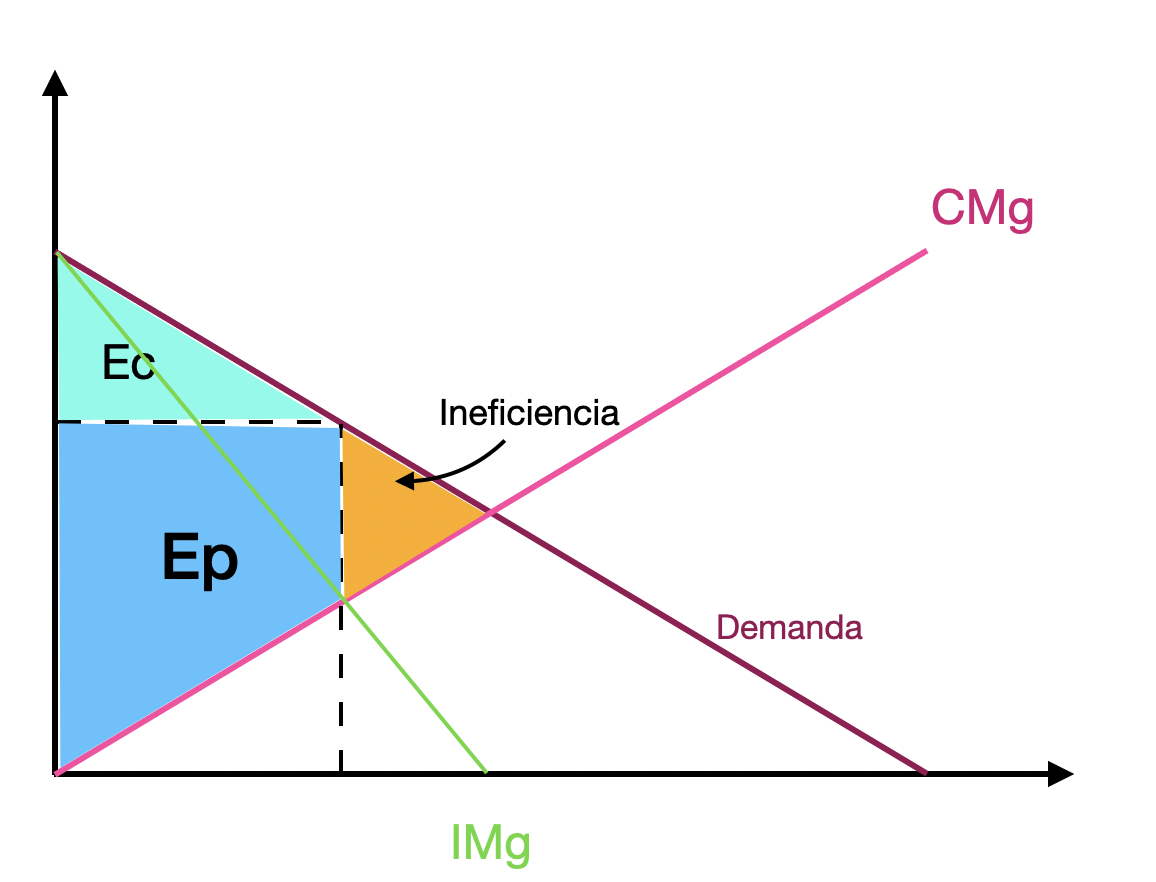
\includegraphics[width=0.65\textwidth]{Modulo_5/ineficencia_monopolio.png}
    \caption{Curva del monopolio. Ec es el excedente consumidor y Ep el excedente del productor}
    \label{fig:inef_monopo}
\end{figure}

El área bajo la curva de demanda hasta cierta cantidad $Q$ es el beneficio total de la sociedad al producirse $Q$ unidades del bien.\\

El área bajo la curva de costos marginales es el costo para la sociedad de producir esas $Q$ unidades.\newline
El excedente social, entonces, es el área entre estas dos curvas, que se maximiza en el punto que se intersectan.\\

Sin embargo el monopolio produce en la intersección de la curva de ingreso marginal con la de costo marginal: el área naranja entre ambas es el excedente social que se pierde, o la ineficiencia que genera el monopolio.\\ 

El excedente de un consumidor está dado por la diferencia entre el precio que estaría dispuesto a pagar y el precio que realmente se cobra.

\subsection{Monopolios naturales}
Hay ciertos mercados que se consideran monopolios naturales, por presentar elementos que favorecen la existencia de una sola firma. Algunos de estos elementos son:

\begin{itemize}
    \item[$\circ$] Barreras de entrada, por ejemplo costos de instalación muy elevados (e.g. compañias de electricidad)
    
    \item[$\circ$] Escasos niveles de sustitución
    
    \item[$\circ$] Derechos de propiedad o patentes
\end{itemize}

A causa de lo anterior, muchas veces el Estado u otra entidad reguladora decide permitir que ciertas firmas actúen como monopolios, normando ciertos aspectos de su quehacer, por ejemplo fijando sus precios.
\newpage